\documentclass[11pt, a4paper]{article}

% --- 1. Paquetes Base y Tipografía ---
\usepackage[T1]{fontenc}
\usepackage[utf8]{inputenc}
\usepackage{lmodern} 
\usepackage{microtype} 

% --- 2. Márgenes y Espaciado ---
\usepackage[margin=1in]{geometry} 
\usepackage{setspace}
\onehalfspacing 

% --- 3. Gráficos, Matemáticas y Tablas ---
\usepackage{graphicx}
\usepackage{subcaption}
\usepackage{amsmath, amssymb, amsthm} 
\usepackage{booktabs} 
\usepackage{tabularx}
\usepackage{xcolor}

% --- 4. Enlaces interactivos ---
\usepackage[colorlinks=true, allcolors=blue]{hyperref}

% --- 5. Información del Documento ---
\title{\textbf{Tarea 2}}
\author{Mariano Fernández}
\date{\today}

\begin{document}

\maketitle

\tableofcontents
\newpage

\section{Introducción}

Este informe presenta los resultados y el análisis correspondientes a la Tarea 2 del 
curso \textit{Introducción a la Ciencia de Datos}. Esta tarea es la continuación de 
la Tarea 1, donde se utiliza el mismo dataset \textit{All the News 2.1 – Component One}.
El dataset contiene artículos en inglés de distintos medios de prensa, con información 
como el título, cuerpo del artículo, fecha de publicación y medio de prensa. 
La implementación de esta tarea se encuentra en el repositorio de GitHub 
\href{https://github.com/MarianoFernandez0/IntroCD}{https://github.com/MarianoFernandez0/IntroCD}.


\section{Dataset y representación numérica de texto}
\subsection{Preparación del dataset}

Para este estudio se utiliza un subconjunto del dataset original, 
formado por las publicaciones de los tres medios de prensa más representados: 
\textit{Reuters}, \textit{The New York Times} y \textit{CNBC}. 
Luego se aplicó la función \texttt{clean\_text} (visto en la Tarea 1) sobre la columna 
del cuerpo del artículo con el objetivo de estandarizar el texto.

Los conjuntos de Train y Test se generaron utilizando una partición estratificada, 
asignando un 30\% de los datos al conjunto de Test y un 70\% al conjunto de Train, 
se utilizó una semilla de 42 para garantizar la reproducibilidad. 
El resultado es de 10425 artículos para entrenamiento y 4469 para prueba, manteniendo 
la proporción de las clases en ambos conjuntos.

\subsection{Balance de clases}

En la figura \ref{fig:class_distribution} se muestra la distribución de clases del dataset,
separando en el conjunto de Train y el conjunto de Test. Se observa que la proporción
se mantiene en aproximadamente igual para ambos conjuntos con un 63\% de artículos de \textit{Reuters},
19\% de \textit{The New York Times} y 18\% de \textit{CNBC}.
Esto también muestra un desbalance claro donde la mayoría de los artículos pertenecen a \textit{Reuters}.

\begin{figure}[h]
    \centering
    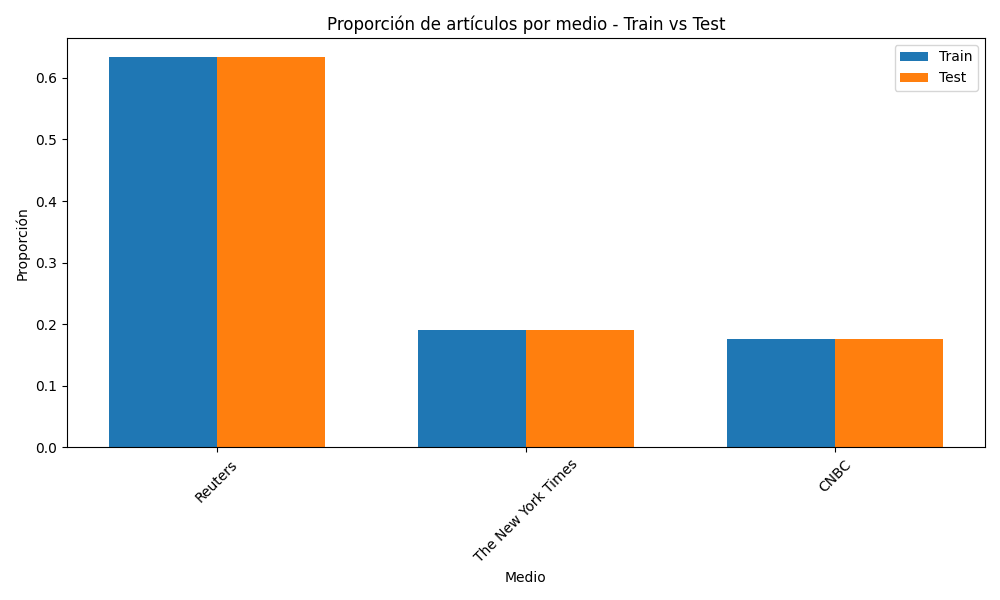
\includegraphics[width=0.8\textwidth]{figures/class_distribution.png}
    \caption{Distribución de clases}
    \label{fig:class_distribution}
\end{figure}

\subsection{Representación Bag of Words}

Para poder entrenar un modelo de clasificación sobre datos de texto es necesario transformarlos 
a una representación numérica que pueda ser procesada por dichos algoritmos. 
Un posible método es \textit{Bag of Words} (BoW), que consiste en primero definir 
el vocabulario del conjunto de entrenamiento, es decir, todas las palabras únicas que aparecen 
en él. Luego, cada artículo se representa por un vector de longitud igual al tamaño del 
vocabulario, donde cada posición indica la cantidad de veces que la palabra correspondiente 
aparece en el texto. El resultado es una matriz de N × M, donde N es el número de artículos 
y M es el tamaño del vocabulario. 

Por ejemplo, si el conjunto de datos es: 
\begin{verbatim}
    "london reuters the world"
    "london aug 8 reuters"
\end{verbatim}
El vocabulario sería: \texttt{["london", "reuters", "the", "world", "aug", "8"]} 
y la representación BoW de cada artículo sería:
\begin{verbatim}
    [1, 1, 1, 1, 0, 0]
    [1, 1, 0, 0, 1, 1]
\end{verbatim}

En el caso particular del dataset utilizado, el tamaño del vocabulario es de 87044 palabras únicas,
lo que resulta en una matriz de 10425 × 87044 para el conjunto de entrenamiento y 4469 × 87044 
para el conjunto de prueba. Si la matriz de entrenamiento se almacenara en un array sin ninguna 
optimización, ocuparía 10425 × 87044 × 4 bytes (asumiendo enteros de 32 bits) lo que equivale
aproximadamente a 3.4 GB de memoria. Dado que para un artículo en particular solo van a aparecer
muy pocas palabras del vocabulario, la mayoría de los campos de la matriz serán cero y el 
resultado es una matriz muy dispersa. Scikit-learn utiliza una representación de matriz dispersa 
que solo almacena los valores no nulos, lo que reduce significativamente el uso de memoria. 
En este caso la matriz de entrenamiento solo ocupa aproximadamente 25.30 MB de memoria.

\subsection{Representación TF-IDF}

Simplemente usar BoW como representación del texto puede llevar a que se pierda mucha información,
una desventaja es que solo se cuenta la cantidad de veces que aparece una palabra pero no se tiene
en cuenta el orden o la relación con palabras vecinas. Como forma de capturar parte de esta 
información se suele utilizar lo que se conoce como N-gramas, que son secuencias de N palabras 
consecutivas.
Por ejemplo si se utiliza N=2, se van a contar no solo las palabras individuales sino también 
las secuencias de dos palabras consecutivas, logrando así capturar contexto local.
Esto tiene un efecto importante en el tamaño del vocabulario, ya que cada par de palabras va 
a representar una nueva feature, lo que hace que incremente el tamaño de la matriz de features 
y el uso de memoria.

Otro punto débil de la representación BoW es que el conteo absoluto de palabras hace que el largo
del texto tenga un impacto grande en la representación, cuando lo relevante es el contenido o tema
del artículo. A esto se suma que las palabras más representadas van a ser las palabras más comunes
en el idioma, y seguramente no aporten mucha información relevante para la tarea de clasificación.
Para solucionar esto se suele utilizar la representación 
\textit{Term Frequency - Inverse Document Frequency} (TF-IDF), que consiste en dos etapas: 
primero normalizar el conteo de palabras por el largo del texto (TF) y segundo multiplicar 
por un factor que penaliza las palabras que aparecen en muchos artículos (IDF).

\begin{itemize}
    \item $\text{TF} = \frac{\text{count}}{\text{total}}$
    \item $\text{IDF} = \log \frac{N}{n}$, donde $N$ es la cantidad de artículos 
    y $n$ la cantidad de artículos donde aparece la palabra.
    \item $\text{TF-IDF} = \text{TF} \times \text{IDF}$
\end{itemize}

En este estudio se utiliza la implementación de la librería Scikit-learn, que es una 
variante de la definición anterior. En particular se agrega un suavizado a la definición 
de IDF para evitar valores extremos para palabras muy poco comunes y que términos 
presentes en todos los documentos no tengan IDF nulo:
\begin{itemize}
    \item $\text{IDF} = \log \frac{1+N}{1+n} + 1$
\end{itemize}
Además en lugar de normalizar TF por el total de palabras del documento, se utiliza la 
norma L2 sobre el vector resultante, de forma de que todos los vectores tengan norma 1. 

\subsection{PCA sobre TF-IDF}

Una forma de visualizar la representación TF-IDF es utilizando PCA para reducir la dimensionalidad
de los datos a 2 dimensiones. En la figura \ref{fig:pca_tfidf} se muestra el resultado de aplicar 
PCA sobre la matriz TF-IDF del conjunto de entrenamiento, cada punto representa un artículo y su 
color el medio de prensa al que pertenece. Se puede observar que en su mayoría los artículos de
\textit{Reuters} se pueden separar bastante bien de los de \textit{The New York Times} pero 
\textit{Reuters} y \textit{CNBC} tienen un overlap muy grande, y por lo menos en esta visualización
no son separables. De todos modos la representación de PCA es una simplificación grande del 
problema y es posible que viéndolo en un espacio de mayor dimensión los datos sí sean separables. 
Como argumento a favor de este punto, en la figura \ref{fig:pca_variance} se muestra la varianza 
explicada acumulativa según la cantidad de componentes que se toman, y las primeras dos 
componentes solo representan aproximadamente el 4\% de la varianza total.

\begin{figure}[h]
    \centering
    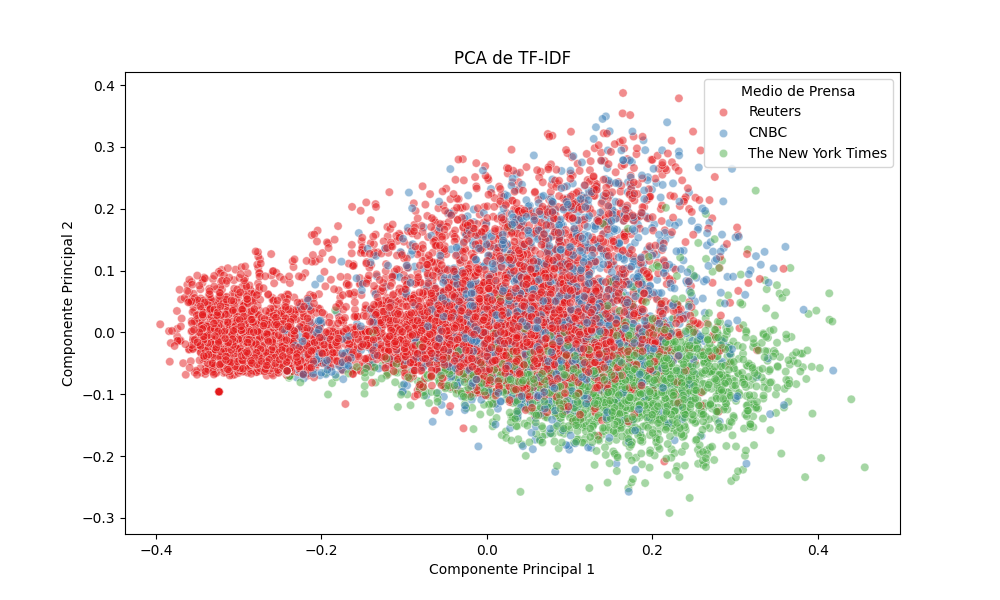
\includegraphics[width=0.8\textwidth]{figures/pca_tfidf.png}
    \caption{PCA sobre TF-IDF}
    \label{fig:pca_tfidf}
\end{figure}


\begin{figure}[h]
    \centering
    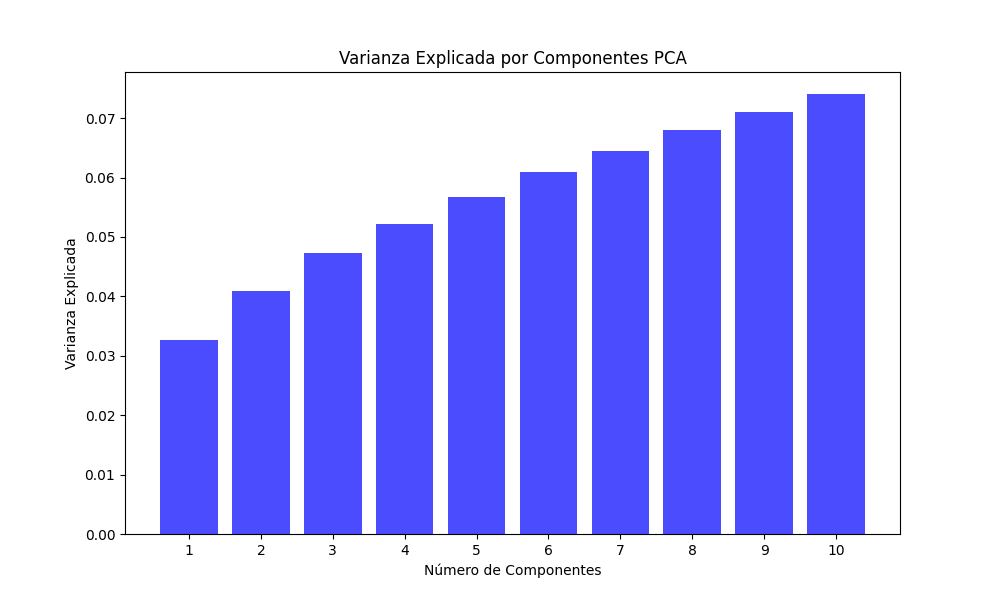
\includegraphics[width=0.8\textwidth]{figures/explained_variance.png}
    \caption{Varianza explicada en PCA por cantidad de componentes}
    \label{fig:pca_variance}
\end{figure}

También se estudió cómo variaba la representación de PCA modificando el preprocesamiento de los 
datos, los resultados se pueden ver en la figura \ref{fig:pca_comparison}.
La forma de los clusters tiene algunas variaciones pero el patrón general se mantiene, en 
particular en todos los casos los artículos de \textit{Reuters} parecen ser separables en dos 
conjuntos diferentes, uno bastante alejado al resto de los medios y fácil de separar y otro que 
en esta proyección es indistinguible de \textit{CNBC}. Lo primero puede explicarse porque muchos
artículos de \textit{Reuters} contienen plantillas que facilitan la separación, como son los
artículos de tipo \textit{BRIEF}, además la separación parece estar más marcada cuando no se usa IDF
probablemente por el peso del largo de los artículos. Por otro lado, una posible explicación del 
overlap entre \textit{Reuters} y \textit{CNBC} que también se observa en todos los casos 
puede ser lo visto en la Tarea 1, donde se concluyó que muchos artículos de \textit{CNBC} 
son realmente artículos de \textit{Reuters}, pero eso no lo puede explicar por completo, ya que de 
ser así se podría ver un subconjunto de artículos de \textit{CNBC} que se separa del resto.
Para confirmar estas hipótesis sería interesante agregar los filtros propuestos en el informe
de la Tarea 1 y ver si los resultados de PCA cambian.

Comparando las figuras \ref{fig:pca_a} y \ref{fig:pca_b} se puede ver que filtrar las stop words
parece tener un efecto positivo en la separación de los clusters, esto tiene sentido si se 
considera que aplicar este filtro resulta en que los artículos estén representados por palabras
más relevantes y diferentes entre medios, lo que resulta en features más separables.
Por otro lado agregar bigramas (figura \ref{fig:pca_c}) no parece tener un gran efecto en la 
separación de los clusters aunque es importante notar que usar n-gramas aumenta la dimensionalidad del
problema mientras que esta proyección reduce la dimensionalidad a solo 2, puede ser que sea necesario 
un espacio de mayor dimensión para que se vea el efecto de los bigramas.
Como ya se vio, quitar la ponderación IDF (figura \ref{fig:pca_d}) parece dejar un subconjunto de 
artículos de \textit{Reuters} más separado del resto, pero parece empeorar la separación de los otros 
clusters.

\begin{figure}[h]
    \centering
    \begin{subfigure}[b]{0.45\textwidth}
        \centering
        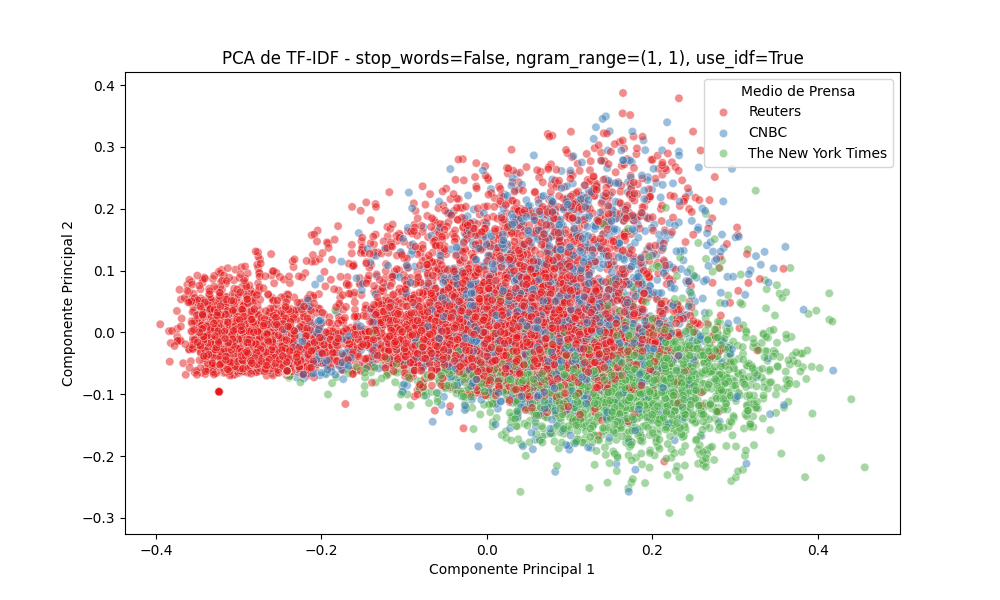
\includegraphics[width=\textwidth]{figures/pca_tfidf_0.png}
        \caption{Base (sin filtrar stop words, unigramas, IDF=True)}
        \label{fig:pca_a}
    \end{subfigure}
    \hfill
    \begin{subfigure}[b]{0.45\textwidth}
        \centering
        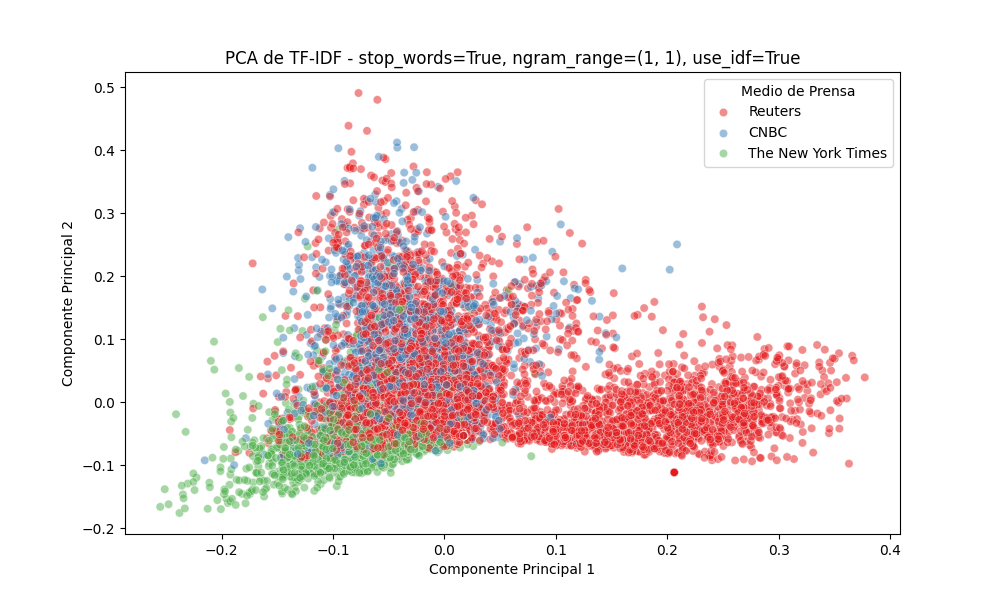
\includegraphics[width=\textwidth]{figures/pca_tfidf_1.png}
        \caption{Filtrando stop words, unigramas, IDF=True}
        \label{fig:pca_b}
    \end{subfigure}

    \vspace{0.5cm}

    \begin{subfigure}[b]{0.45\textwidth}
        \centering
        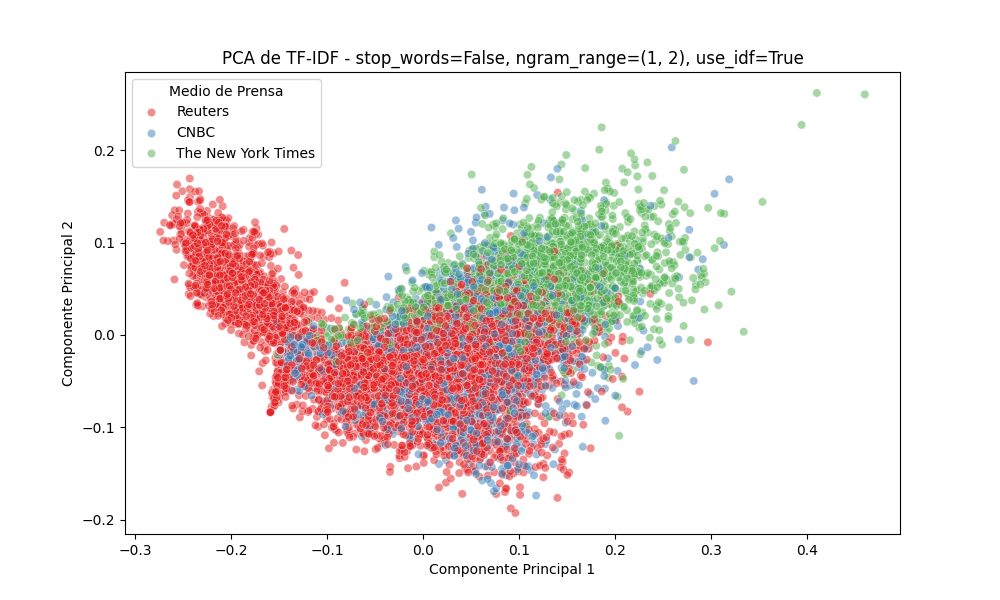
\includegraphics[width=\textwidth]{figures/pca_tfidf_2.png}
        \caption{Sin filtrar stop words, con bigramas (ngram\_range=(1,2)), IDF=True}
        \label{fig:pca_c}
    \end{subfigure}
    \hfill
    \begin{subfigure}[b]{0.45\textwidth}
        \centering
        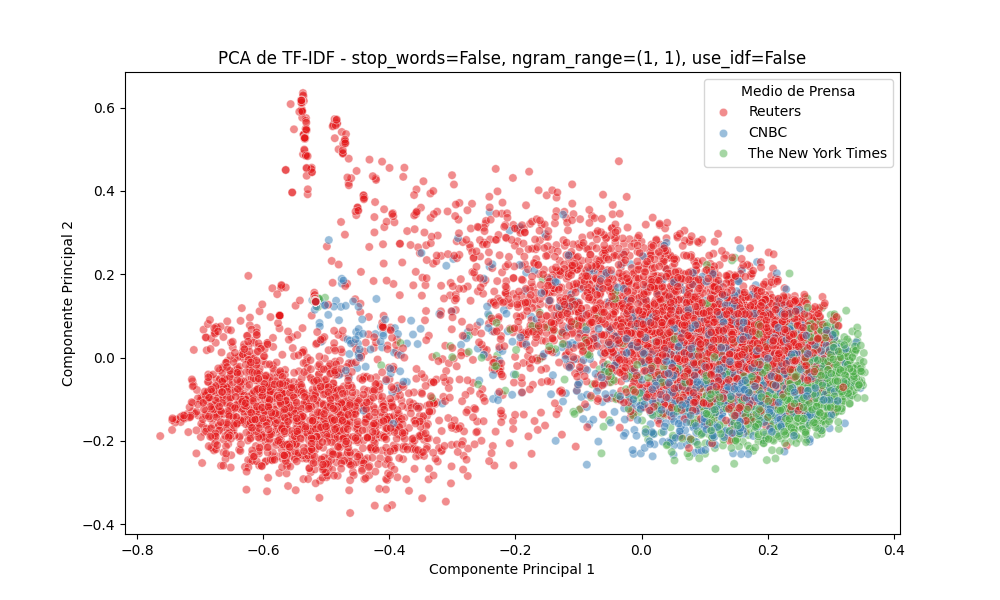
\includegraphics[width=\textwidth]{figures/pca_tfidf_3.png}
        \caption{Sin filtrar stop words, unigramas, sin ponderación IDF (use\_idf=False)}
        \label{fig:pca_d}
    \end{subfigure}

    \caption{Comparación de PCA sobre distintas configuraciones del vectorizador de texto.}
    \label{fig:pca_comparison}
\end{figure}


\section{Entrenamiento y evaluación de modelos}
\subsection{Multinomial Naive Bayes}

A partir de la representación TF-IDF se entrena un modelo Multinomial Naive Bayes
en el conjunto de entrenamiento, con los parámetros predeterminados y se evalúa 
en el conjunto de prueba donde se obtiene un accuracy del 70.13\%. Esto quiere
decir que el modelo es capaz de clasificar correctamente el 70\% de los artículos
del conjunto de test, el problema es que este número puede ocultar problemas con
el modelo, por ejemplo como se vio anteriormente \textit{Reuters} predomina en el dataset por 
lo que también va a tener un peso más grande en el cálculo del accuracy, si el modelo prediciera
siempre \textit{Reuters} ya obtendría un 63\% de acccuracy.


Para tener una mejor visión del desempeño del modelo, en la figura \ref{fig:confusion_matrix} 
se muestra la matriz de confusión en el conjunto de prueba que se acompaña con la tabla de 
métricas \ref{tab:metrics_nb}, como era de esperarse el modelo tiende a clasificar un artículo
como perteneciente a \textit{Reuters}, por esto su Recall en \textit{Reuters} es casi 1, solo 3/2830 se clasifican
erróneamente como otra clase. El problema aparece al ver que la Precision de la clase \textit{Reuters} es 
de 68\%, es decir que de todos los artículos que se predicen como \textit{Reuters} 32\% son de otra clase. 
El efecto es más claro cuando se estudian las métricas de las otras clases, principalmente \textit{CNBC} 
que tiene una precisión de 100\% pero un recall de 1\% eso quiere decir que todos los artículos 
que predice como \textit{CNBC} los predice correctamente pero son solo 8, que representan el 1\% de los 
textos del medio, la gran mayoría de los artículos de \textit{CNBC} se clasifican como \textit{Reuters}. 
Esto coincide con la poca separabilidad entre \textit{Reuters} y \textit{CNBC} que se vio en la
visualización de PCA \ref{fig:pca_tfidf}.

\begin{table}[h]
    \centering
    \begin{tabular}{lccc}
        \hline
        \textbf{Métrica} & \textbf{Reuters} & \textbf{The New York Times} & \textbf{CNBC} \\
        \hline
        Precision & 0.6812 & 0.9614 & 1.0000 \\
        Recall & 0.9989 & 0.3509 & 0.0102 \\
        F1-score & 0.8100 & 0.5142 & 0.0201 \\
        \hline
    \end{tabular}
    \caption{Resultados del modelo Multinomial Naive Bayes base}
    \label{tab:metrics_nb}
\end{table}

\begin{figure}
    \centering
    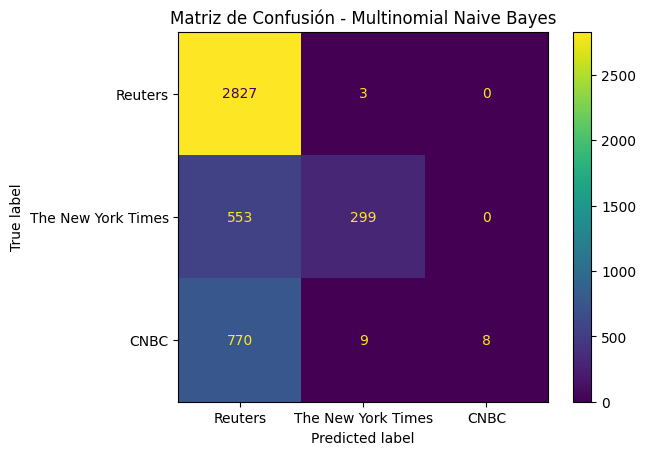
\includegraphics[width=0.8\textwidth]{figures/confusion_matrix_nb.png}
    \caption{Matriz de confusión del modelo Naive Bayes}
    \label{fig:confusion_matrix}
\end{figure}

\subsection{Validación cruzada y búsqueda de hiperparámetros}

Hasta el momento se entrenó solo un modelo sin modificar los parámetros predeterminados pero una 
parte importante del entrenamiento es la búsqueda de hiperparámetros del modelo, que pueden afectar
considerablemente el desempeño final. Una consideración clave a tener es que no se puede usar el 
mismo conjunto de test para esta búsqueda porque podría llevar a un sobreajuste en este conjunto
y las métricas de desempeño no representen la realidad del problema. Para solucionar este
problema se suelen usar dos estrategias: 


En lugar de solo particionar el conjunto en entrenamiento y prueba, se vuelve a particionar el 
conjunto de entrenamiento para obtener el conjunto de validación, este es similar al conjunto 
de Test que se usa para comparar diferentes configuraciones del modelo (hiperparámetros) y luego 
de obtener la mejor se evalúa en el conjunto de prueba para obtener una estimación del desempeño 
del modelo. El problema con esa estrategia es que se reduce mucho la cantidad de datos de 
entrenamiento y los mejores hiperparámetros elegidos dependen mucho del split realizado, por esto 
otra estrategia muy utilizada es validación cruzada donde se repite N veces la estrategia anterior. 
Se generan N splits, de forma de los N conjuntos de validación resultantes no tengan overlap y la 
suma de todos cubra todo el conjunto de train, luego para cada configuración se repite el 
entrenamiento en cada uno de los N splits y se reportan los resultados finales en cada partición. 
Como paso final se eligen los hiperparámetros que obtuvieron el mejor desempeño promedio en los N splits 
y se entrena un modelo con ellos, utilizando todo el conjunto de entrenamiento.

En la figura \ref{fig:grid_search_results} se muestra el resultado de la búsqueda de hiperparámetros
realizada para el modelo Multinomial Naive Bayes, para todas las combinaciones de los siguientes
hiperparámetros:
\begin{verbatim}
    alpha: [0.1, 0.25, 0.5, 0.75, 1.0]
    fit_prior: [True, False]
\end{verbatim}
Obteniendo un total de 10 configuraciones diferentes. De la gráfica \ref{fig:grid_search_results} 
se concluye que \texttt{alpha=0.1} suele obtener mejores resultados y para ese caso no hay una 
gran diferencia entre si usar \texttt{fit\_prior} o no.

\begin{figure}
    \centering
    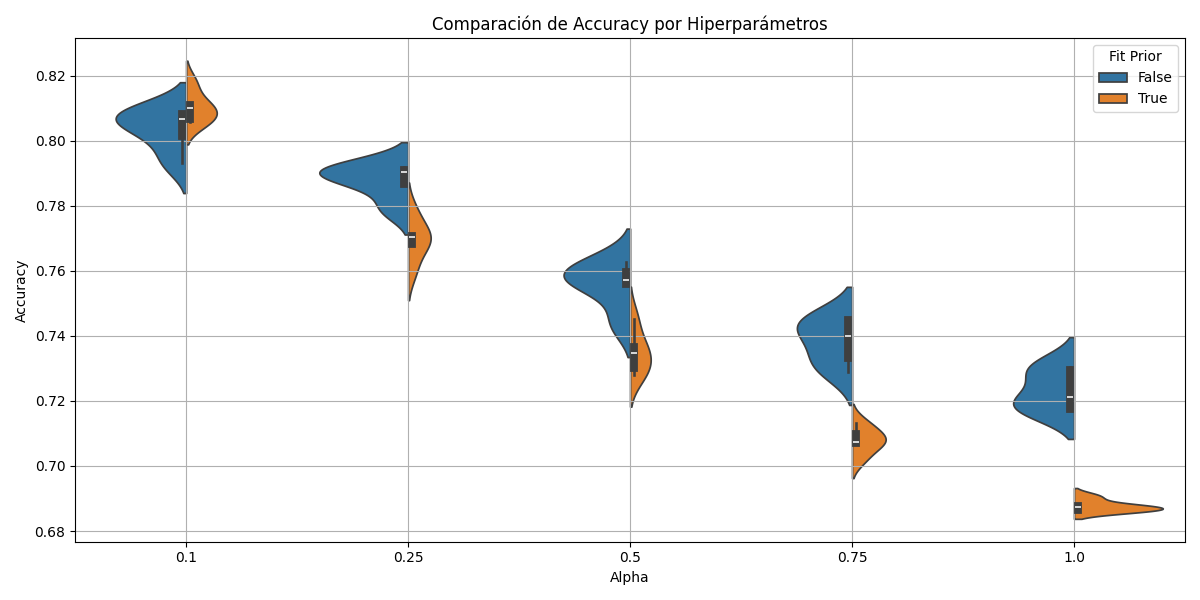
\includegraphics[width=0.8\textwidth]{figures/grid_search_violin.png}
    \caption{Resultados de GridSearchCV}
    \label{fig:grid_search_results}
\end{figure}

\subsection{Entrenamiento con mejores hiperparámetros}

Los mejores hiperparámetros obtenidos de la sección anterior son: \texttt{alpha=0.1} y 
\texttt{fit\_prior=True}, se usan estos parámetros para entrenar el modelo en todo el conjunto 
de train obteniendo un accuracy de 80.47\% en el conjunto de Test, lo que significa una mejora 
de +10 puntos sobre usar los hiperparámetros predeterminados. Además viendo la matriz de 
confusión de la figura \ref{fig:confusion_matrix_best} y las métricas de Precision y Recall 
por medio de la tabla \ref{tab:metrics_best_nb} este modelo ya no presenta tanto el problema de 
clasificar todos los artículos como \textit{Reuters}. El problema que se mantiene es que el Recall de 
\textit{CNBC} aún es muy bajo, 30\%, lo que refuerza la hipótesis que muchos artículos 
de \textit{CNBC} no son separables de los de \textit{Reuters}.

\begin{figure}
    \centering
    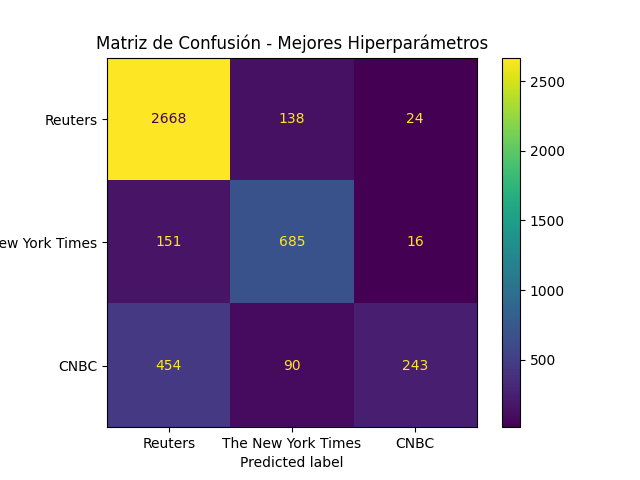
\includegraphics[width=0.8\textwidth]{figures/confusion_matrix_best_nb.png}
    \caption{Matriz de confusión del modelo con mejores hiperparámetros}
    \label{fig:confusion_matrix_best}
\end{figure}

\begin{table}[h]
    \centering
    \begin{tabular}{lccc}
        \hline
        \textbf{Métrica} & \textbf{Reuters} & \textbf{The New York Times} & \textbf{CNBC} \\
        \hline
        Precision & 0.8152 & 0.7503 & 0.8587 \\
        Recall & 0.9428 & 0.8040 & 0.3088 \\
        F1-score & 0.8743 & 0.7762 & 0.4542 \\
        \hline
    \end{tabular}
    \caption{Resultados del modelo con mejores hiperparámetros}
    \label{tab:metrics_best_nb}
\end{table}

\subsection{Random Forest}

Como modelo alternativo a Multinomial Naive Bayes se decidió entrenar un modelo Random Forest, 
que es un modelo de clasificación basado en árboles de decisión. En resumen, en lugar de entrenar
un solo árbol de decisión, se entrenan varios árboles, haciendo modificaciones aleatorias en los 
datos de entrenamiento de cada uno y en las features que se utilizan para cada árbol para asegurar
que cada uno sea diferente. Luego al momento de clasificar un artículo se hace una votación para
obtener la predicción final. 

El uso de Random Forest en lugar de un solo árbol de decisión tiene 
varias ventajas, principalmente suele generalizar mejor ya que un problema de los árboles de decisión 
es que tienden a sobreajustar a los datos de entrenamiento, una pequeña modificación en los datos de 
entrenamiento puede causar grandes cambios en el modelo. 

El modelo se entrenó con los hiperparámetros predeterminados, obteniendo un accuracy de 83.11\% en 
el conjunto de prueba, este resultado ya es mejor que el mejor modelo Naive Bayes con hiperparámetros 
optimizados. 
Cuando se estudia la matriz de confusión se ve un patrón similar al modelo anterior, 
siendo \textit{Reuters} la clase con mejor desempeño, luego \textit{The New York Times} y por último \textit{CNBC} 
con la mayoría de los artículos clasificados como \textit{Reuters}.
\begin{figure}
    \centering
    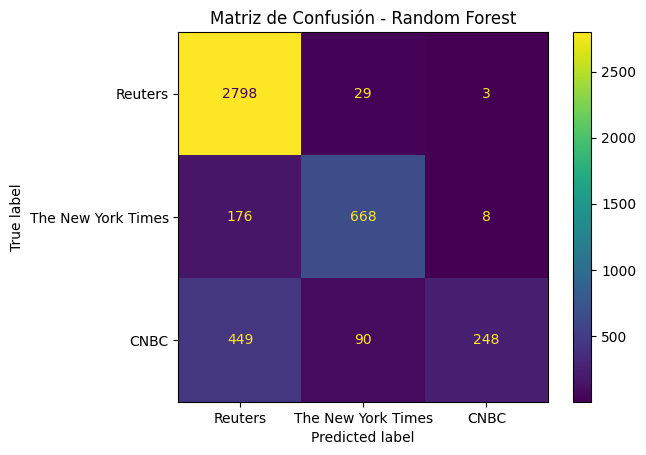
\includegraphics[width=0.8\textwidth]{figures/confusion_matrix_rf.png}
    \caption{Matriz de confusión del modelo Random Forest}
    \label{fig:confusion_matrix_rf}
\end{figure}

\subsection{Cambio de medio de prensa}

Como gran parte de los problemas vistos en este informe surgen por el desbalance causado por el número de artículos 
de  \textit{Reuters} o un problema en la clasificación de los datos de \textit{CNBC} vs \textit{Reuters}, 
se consideró interesante elegir un subconjunto alternativo del dataset que no contenga \textit{Reuters}.

Se seleccionaron los top 3 medios de prensa del dataset (descartando \textit{Reuters}), obteniendo los
siguientes medios: \textit{The New York Times}, \textit{CNBC} y \textit{The Hill}.
En la figura \ref{fig:class_distribution2} se puede observar como la distribución de clases es 
mucho más pareja que en el conjunto original representado por la figura \ref{fig:class_distribution}.

El nuevo conjunto de datos parece definir una tarea más fácil para el modelo, una posible razón es que
al eliminar \textit{Reuters} se reduce bastante el ruido en los datos. El modelo Multinomial Naive Bayes,
entrenado con los hiperparámetros predeterminados, obtuvo un accuracy de 87\% en el conjunto de prueba. 
Además en la matriz de confusión \ref{fig:confusion_matrix_nb_change} se puede ver un buen desempeño,
sobre todo al separar \textit{The New York Times} y \textit{The Hill}, esto puede ser la diferencia temática
de los medios. Por otro lado todavía se puede ver que gran parte de los artículos de \textit{CNBC} se siguen clasificando
erróneamente, en este caso la mayoría de los errores son porque el modelo predice \textit{The New York Times}. 

\begin{figure}
    \centering
    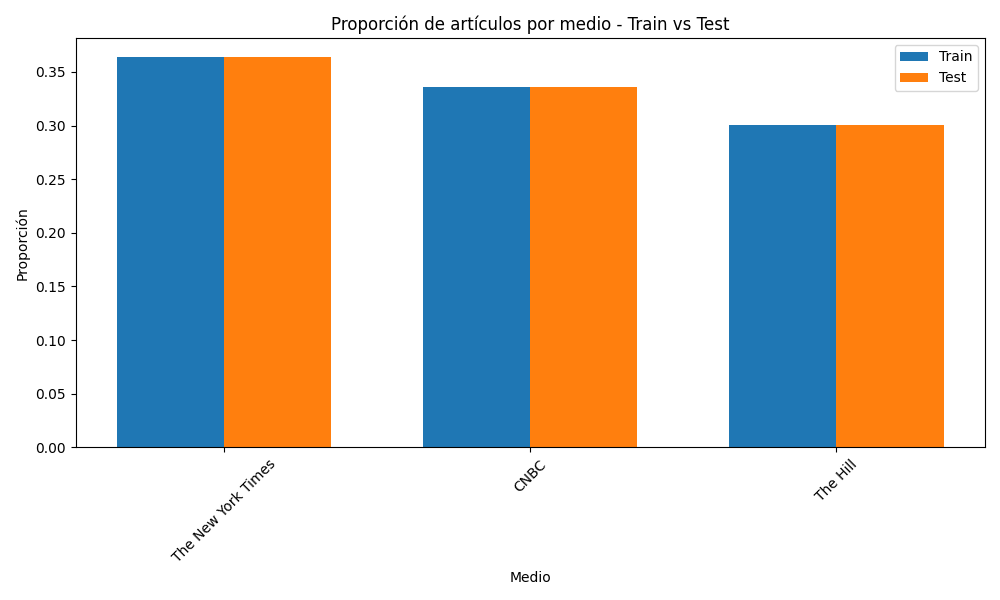
\includegraphics[width=0.8\textwidth]{figures/class_distribution2.png}
    \caption{Distribución por clase para subconjunto alternativo.}
    \label{fig:class_distribution2}
\end{figure}

\begin{figure}
    \centering
    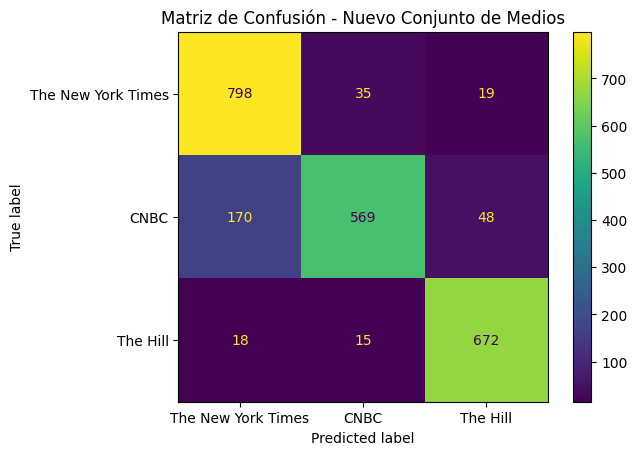
\includegraphics[width=0.8\textwidth]{figures/confusion_matrix_sampled_nb.png}
    \caption{Matriz de confusión del modelo Naive Bayes con cambio de medio de prensa}
    \label{fig:confusion_matrix_nb_change}
\end{figure}

\subsection{Extracción de features alternativa}

La representación TF-IDF mantiene más información que utilizando BoW, pero aún así se 
pierde información importante del texto. Una solución alternativa es utilizar un método que genere
embeddings de palabras, estos suelen ser vectores de mucho menor dimensión que la representación 
TF-IDF y se entrenan para capturar relaciones semánticas entre palabras. Es decir dos embeddings
de palabras que tengan un significado similar van a estar más cerca en el espacio de embeddings.

Un algoritmo muy utilizado para generar embeddings en tareas de texto es Word2Vec, que se entrena 
con un corpus de texto y genera un embedding para cada palabra.

Aplicar Word2Vec sobre el dataset agrega una complejidad extra al problema, ya que ahora para
cada artículo se obtiene una secuencia de embeddings de palabras, en lugar de un vector de largo fijo.
Entonces, para poder entrenar los mismos modelos de clasificación que antes es necesario agregar una etapa 
que lleve estas secuencias de embeddings a un vector de largo fijo. Una forma sería promediar
todos los embeddings de palabras del artículo, para obtener un único vector de features.

Otro enfoque que puede llegar a mejores resultados es utilizar un modelo que tome secuencias 
de largo variable como entrada, como por ejemplo una red neuronal recurrente (RNN) o un modelo
transformer. Estos modelos son más complejos, requieren más tiempo de entrenamiento y más datos 
para generalizar bien, pero pueden hacer un mejor uso de toda la información del texto.

\subsection{Clasificación a nivel de título}

Otro experimento interesante es ver si es posible clasificar el artículo utilizando sólo el título,
es de esperar un desempeño peor que usando todo el cuerpo del artículo ya que la cantidad de 
información es mucho menor. 

A pesar de esto, entrenando un modelo Multinomial Naive Bayes con los 
hiperparámetros predeterminados se obtuvo un 70\% de accuracy en el conjunto de prueba. Esto se podría explicar
en parte por el desbalance en las clases que ya se vio, dado que por cómo se calcula la métrica de accuracy si 
el modelo tiende a predecir \textit{Reuters} la métrica da mejor. 
Esto además es respaldado por la matriz de confusión \ref{fig:confusion_matrix_title} donde se ve que la mayoría de
los artículos son clasificados como \textit{Reuters}.

\begin{figure}
    \centering
    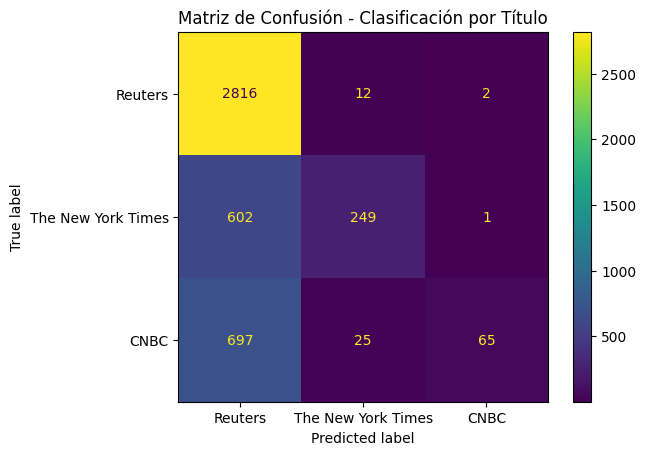
\includegraphics[width=0.8\textwidth]{figures/confusion_matrix_title_nb.png}
    \caption{Matriz de confusión del modelo Naive Bayes con clasificación a nivel de título}
    \label{fig:confusion_matrix_title}
\end{figure}

\end{document}